%!TEX root = ../thesis.tex
% **************************** Define Graphics Path **************************
\ifpdf
\graphicspath{{Chapter5/Figs/Raster/}{Chapter5/Figs/PDF/}{Chapter5/Figs/}}
\else
\graphicspath{{Chapter5/Figs/Vector/}{Chapter5/Figs/}}
\fi

%*******************************************************************************
%****************************** Fifth Chapter *********************************
%*******************************************************************************

\chapter{Experiments and Results}
\label{chapter5}
\hl{todo}
\begin{enumerate}
	\item training experiments
	\item sampling experiments
	\item mention computationally expensive parts!
\end{enumerate}

\section{Learning the rates} 
\begin{figure}
	\centering
	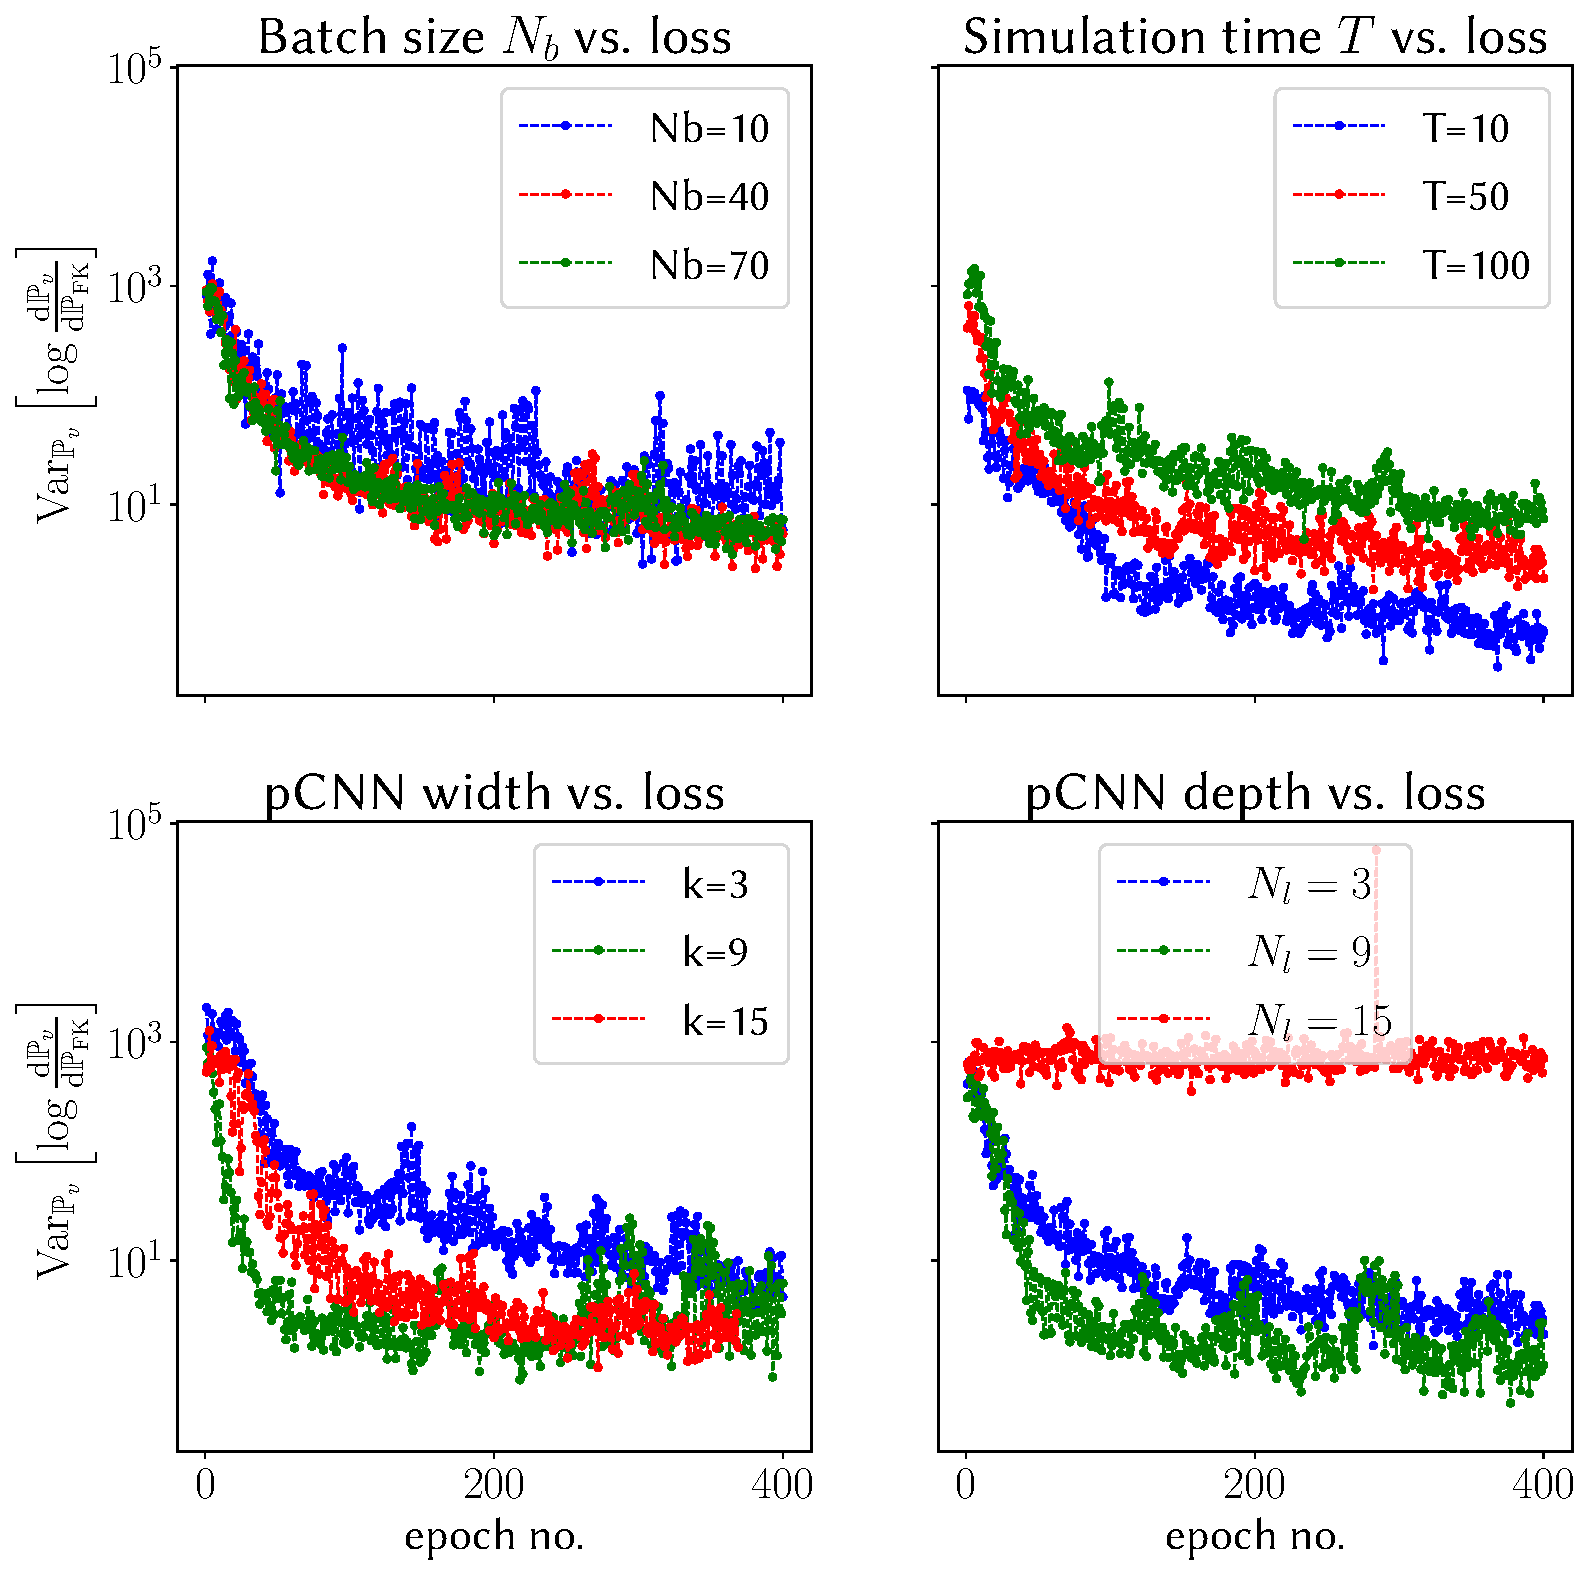
\includegraphics[width=\linewidth]{Chapter5/Figs/Vector/init_test_learning}
	\caption[Initial rate training experiments]{\textbf{Initial rate training experiments}}
	\label{fig:inittestlearning}
\end{figure}

\begin{figure}
	\centering
	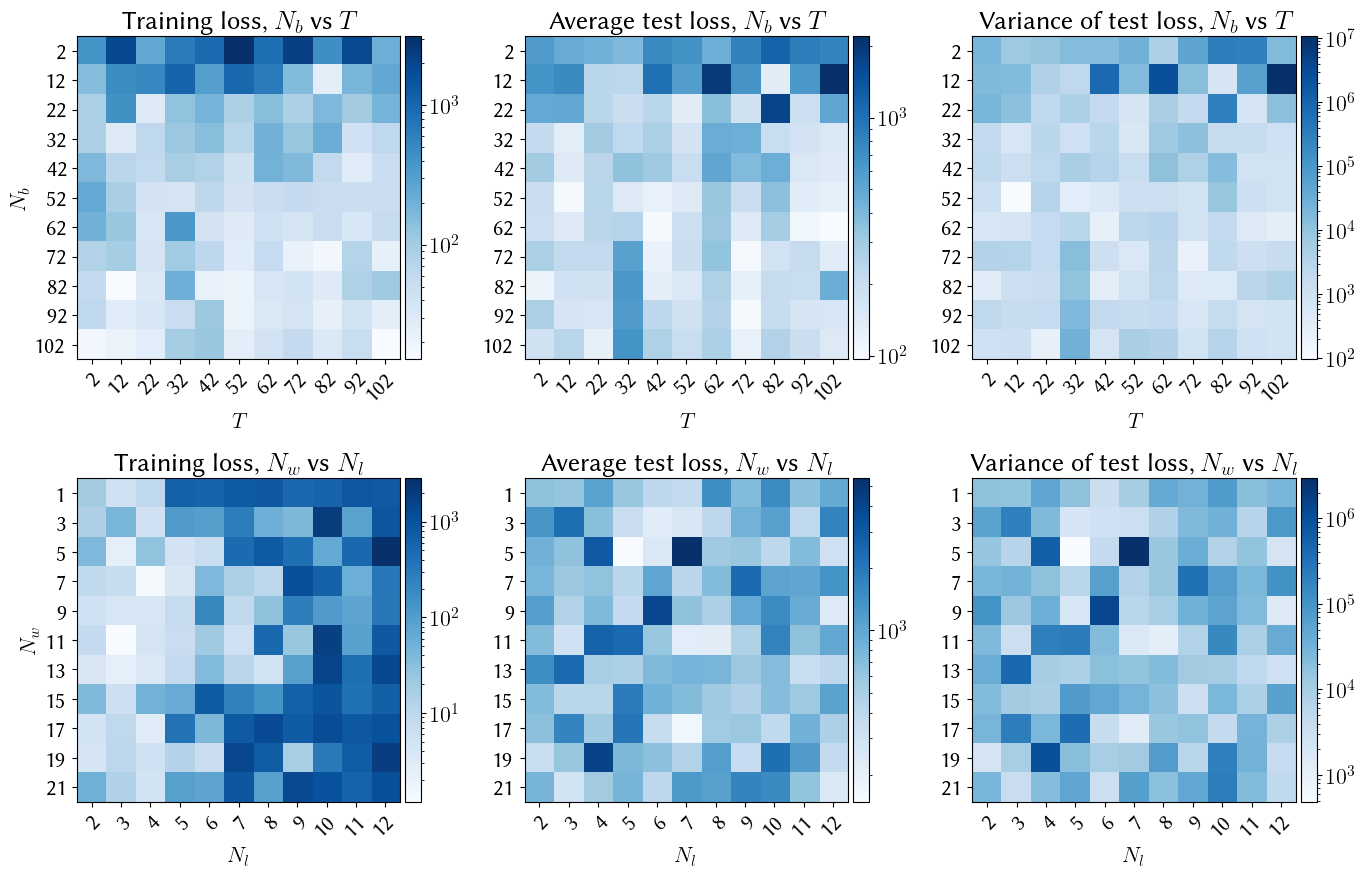
\includegraphics[width=\linewidth]{Chapter5/Figs/Raster/avg_var_loss}
	\caption[Performance of the pCNN for different setups]{\textbf{Performance of the pCNN for different setups.}}
	\label{fig:avgvarloss}
\end{figure}

\begin{figure}
	\centering
	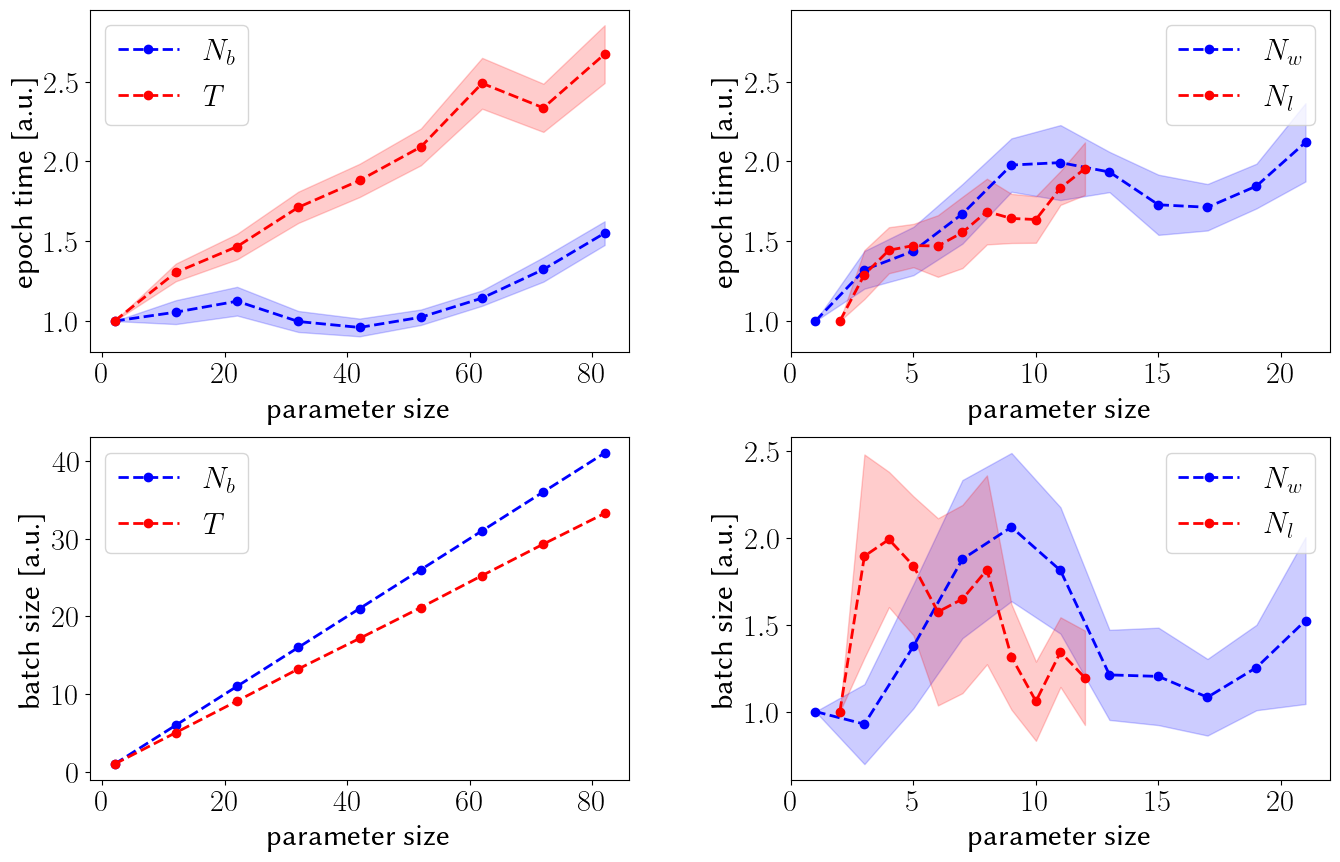
\includegraphics[width=\linewidth]{Chapter5/Figs/Raster/initial_time_space}
	\caption[Time and space complexity of the pCNN]{\textbf{Time and space complexity of the pCNN}}
	\label{fig:initialtimespace}
\end{figure}

%\subsubsection{How does simulation time $T$ and batch size $N_b$ affect the learning of the rates?}
%
%\subsubsection{How do architectural choices of the pCNN limit learning the rates?}
%
%\subsubsection{How does the size of lattice play a role?}
%
%\subsubsection{Can we improve learning by scaling the output of the pCNN?}
%Also mention reshuffling.
%
%\subsubsection{What role does symmetry play in all of this?}

\section{Importance sampling}
\section{Results}
\subsection{Ising model}
\subsubsection{One dimension}
\begin{figure}[H]
	\centering
	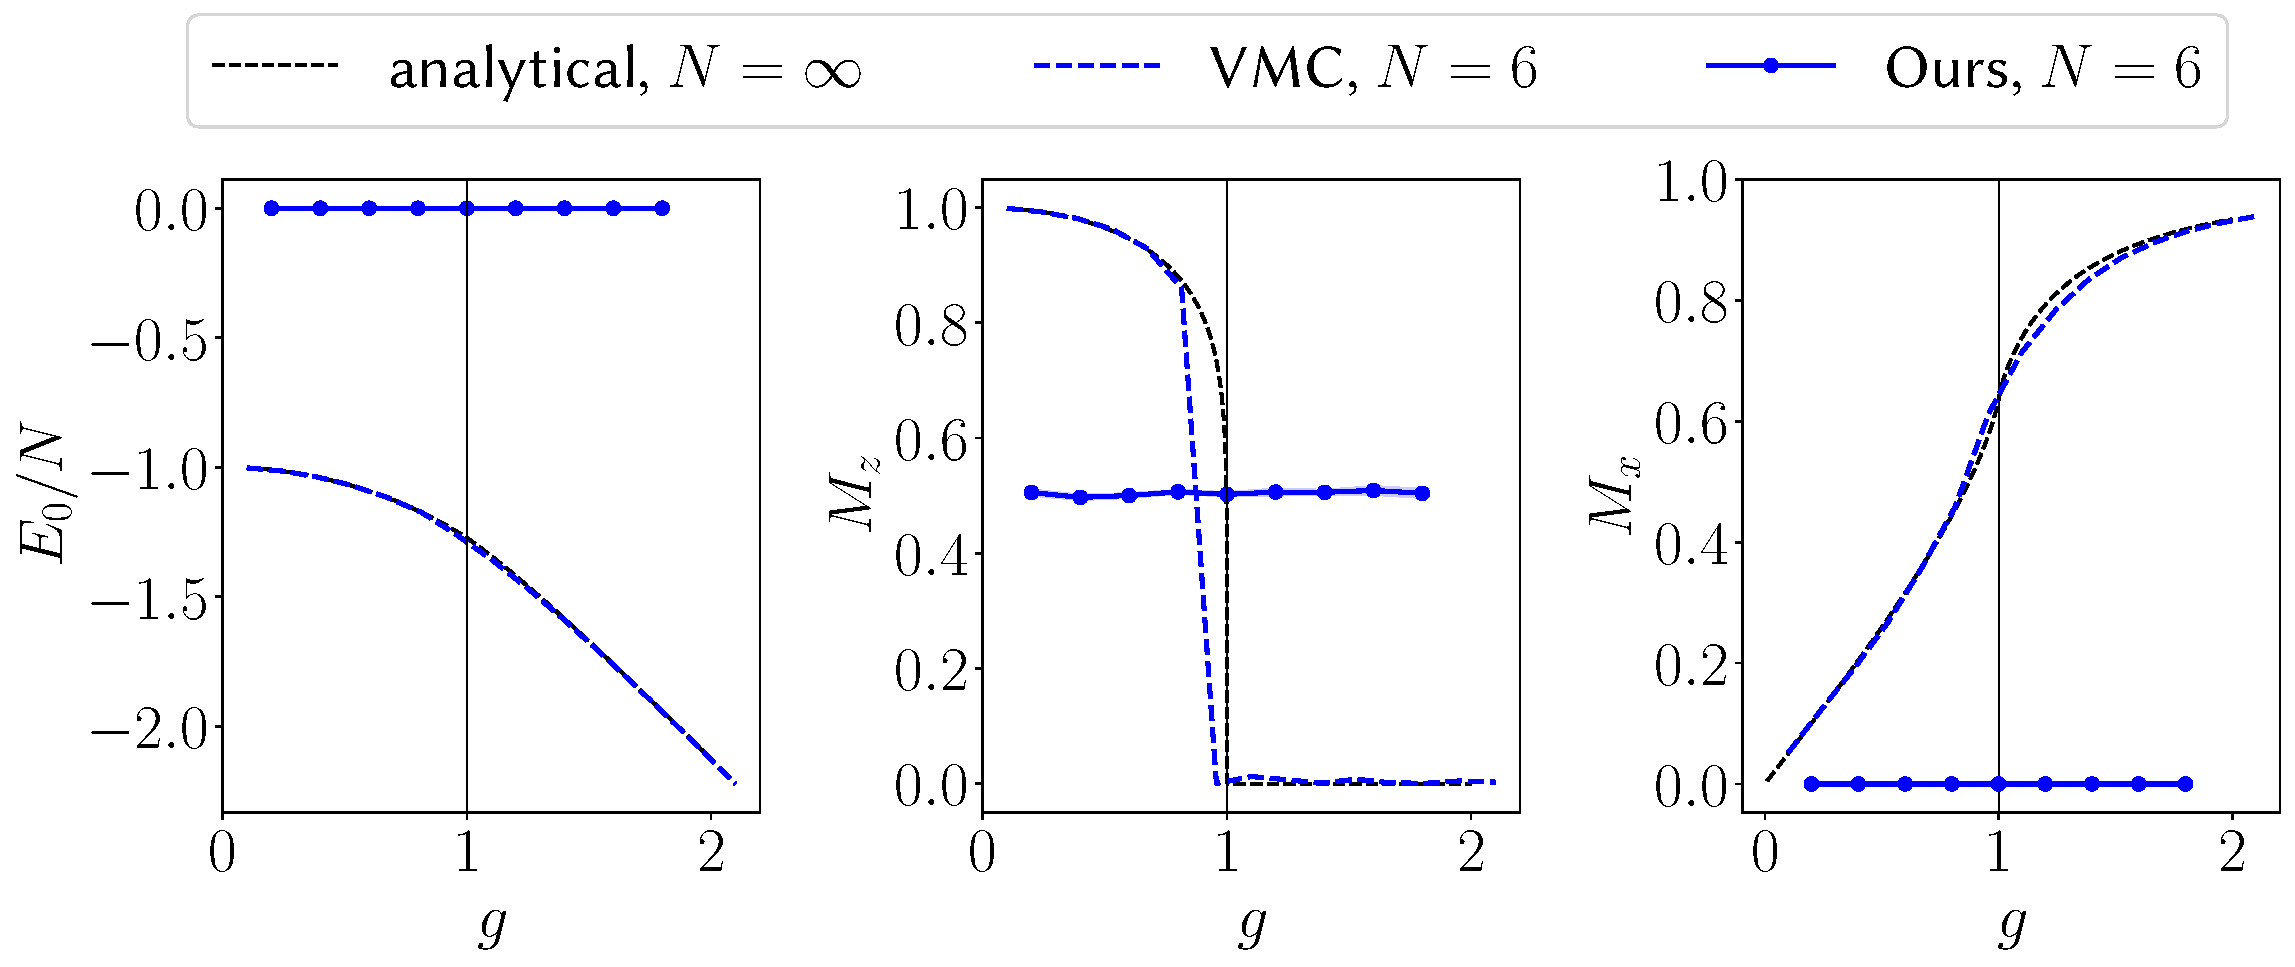
\includegraphics[width=\linewidth]{Chapter5/Figs/Vector/tfim1d_finite_scaling.pdf}
	\caption[TFIM-1d energy and magnetisations]{\textbf{TFIM-1d energy and magnetisation}}
	\label{fig:tfim1d_finite_scaling_properties}
\end{figure}

\begin{figure}[H]
	\centering
	\subfloat{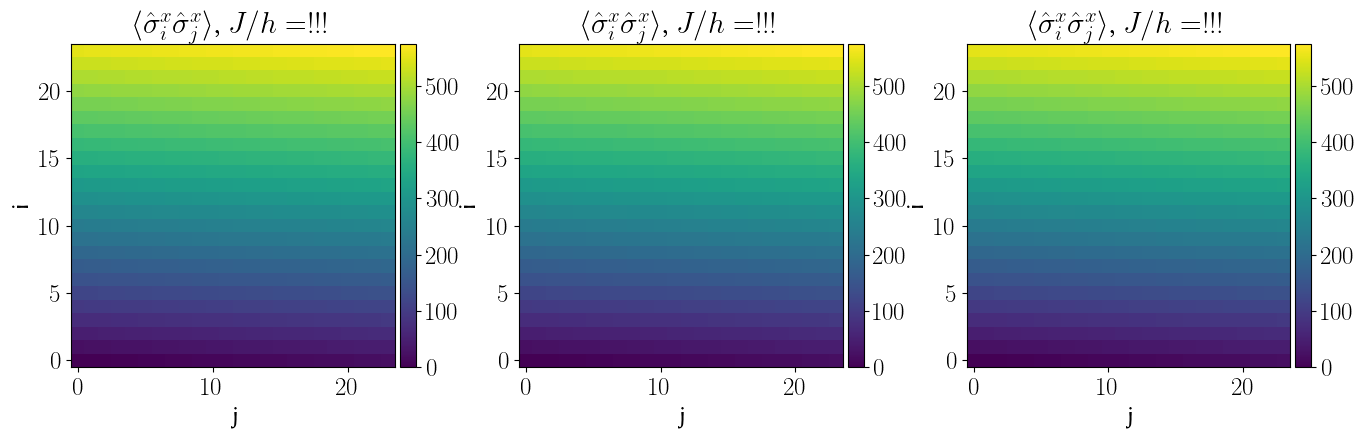
\includegraphics[width=\linewidth]{Chapter5/Figs/Raster/tfim1d-sisj-x.png}} \\
	\subfloat{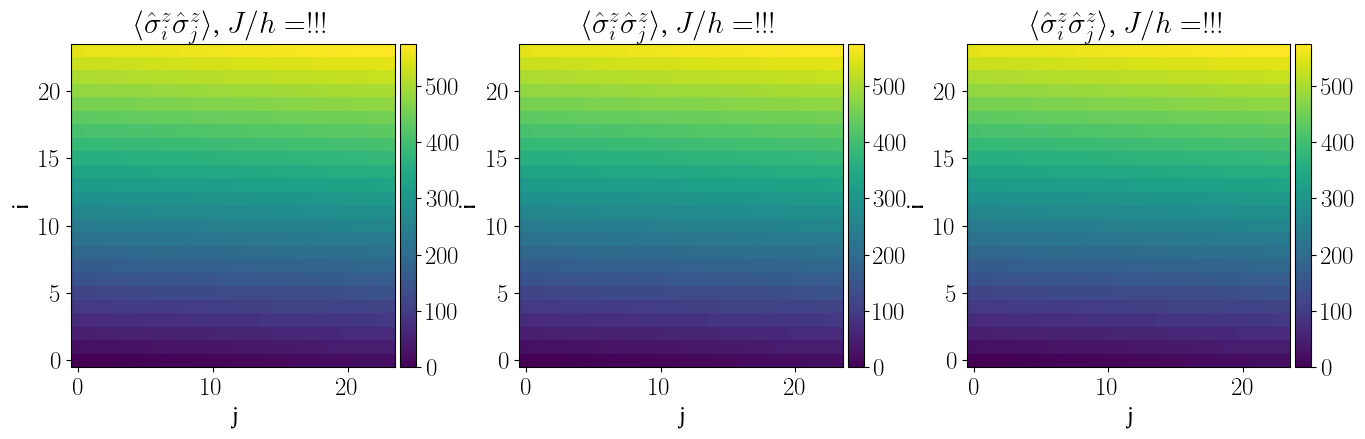
\includegraphics[width=\linewidth]{Chapter5/Figs/Raster/tfim1d-sisj-z.png}}
	\caption[]{\textbf{}}
	\label{fig:tfim1d_sisj}
\end{figure}

\subsubsection{Two dimensions}
\begin{figure}[H]
	\centering
	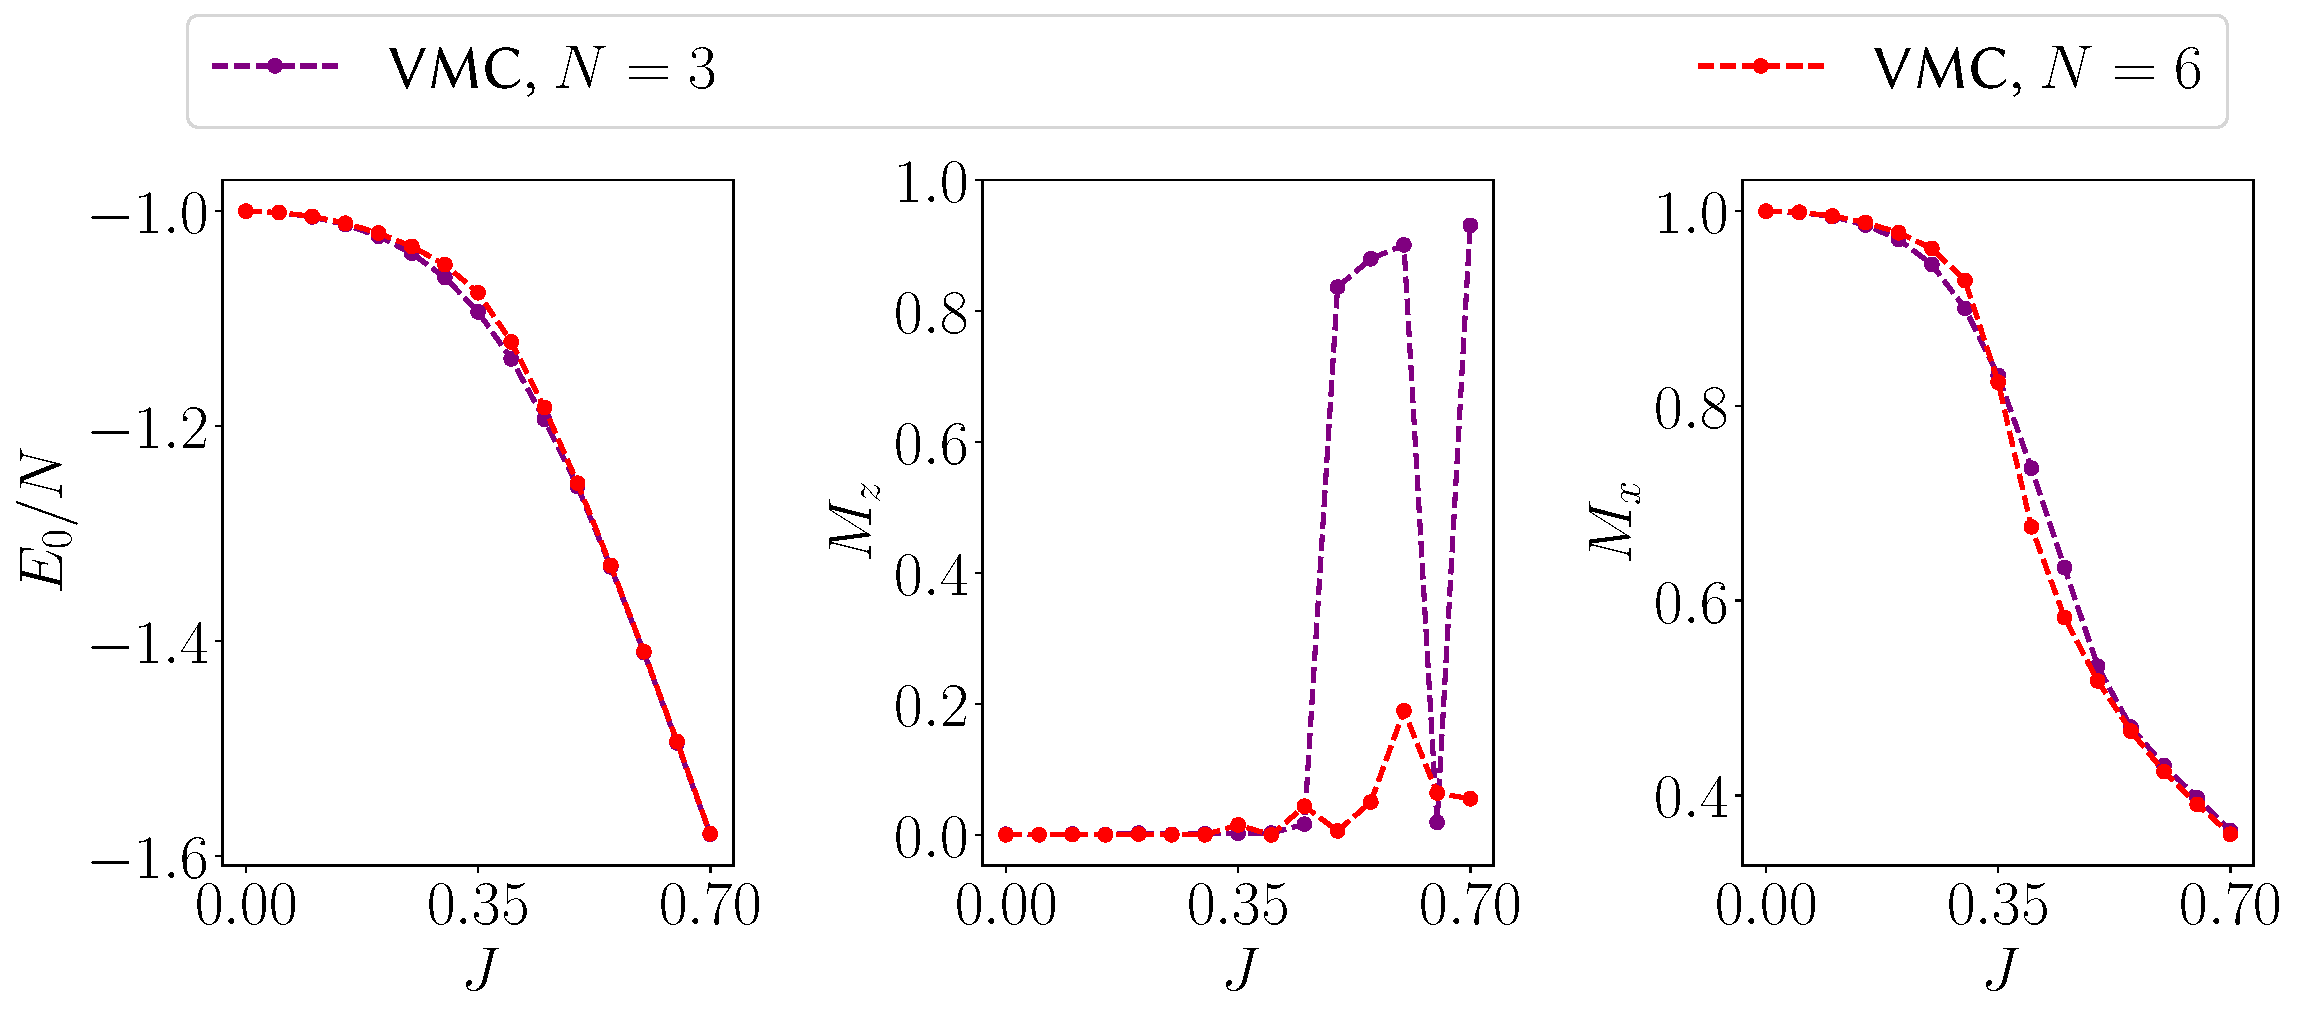
\includegraphics[width=\linewidth]{Chapter5/Figs/Vector/tfim2d_finite_scaling.pdf}
	\caption[TFIM-2d energy and magnetisations]{\textbf{TFIM-2d energy and magnetisation}}
	\label{fig:tfim2d_finite_scaling_properties}
\end{figure}

\newpage
\subsection{XY model}